%% ani.tex
%% Author: Leighton Pritchard
%% Copyright: James Hutton Institute
%% Average Nucleotide Identity

%
\begin{frame}
  \frametitle{Average Nucleotide Identity (ANI)
  \footnote{\tiny{\href{http://dx.doi.org/10.1099/ijs.0.64483-0
}{Goris \textit{et al.} (2007) \textit{Int. J. System. Evol. Biol.} doi:10.1099/ijs.0.64483-0
}}}
  }
  Introduced as an \textit{in silico} substitute for DDH in 2007:
  \begin{columns}[T] 
    \column{.6\textwidth} 
      \begin{itemize}
        \item \textcolor{hutton_green}{70\% identity (DDH) = "gold standard" prokaryotic species boundary}
        \item \textcolor{hutton_blue}{70\% identity (DDH) $\approx$ 95\% identity (ANI)}
      \end{itemize}
    \column{.4\textwidth}
      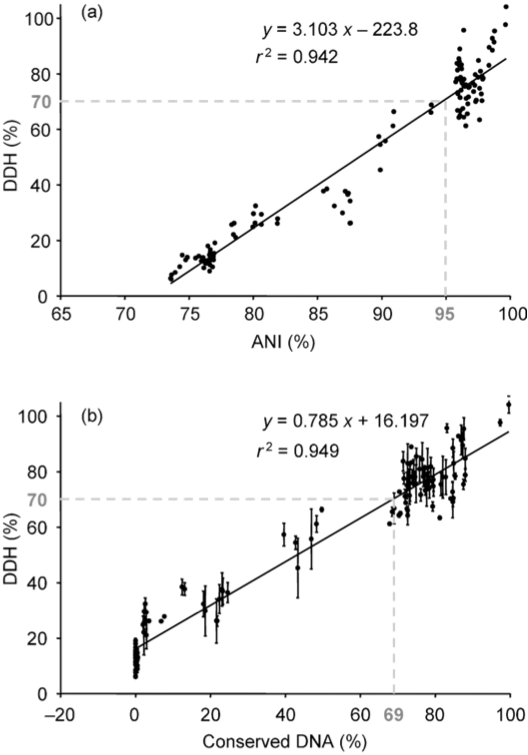
\includegraphics[width=\textwidth]{images/ani_ddh_equiv}
  \end{columns}    
\end{frame}

%
\begin{frame}
  \frametitle{Average Nucleotide Identity (ANI)
  \footnote{\tiny{\href{http://dx.doi.org/10.1099/ijs.0.64483-0
}{Goris \textit{et al.} (2007) \textit{Int. J. System. Evol. Biol.} doi:10.1099/ijs.0.64483-0
}}}
  }
  Original method emulated physical experiment:
  \begin{columns}[T] 
    \column{.6\textwidth} 
      \begin{enumerate}
        \item \textcolor{hutton_green}{break genome into 1020nt fragments}
        \item \textcolor{hutton_blue}{align all fragments with BLASTN}
        \item \textcolor{hutton_purple}{ANI = mean identity of all matches with $>30\%$ identity, $>70\%$ coverage}
      \end{enumerate}
    \column{.4\textwidth}
      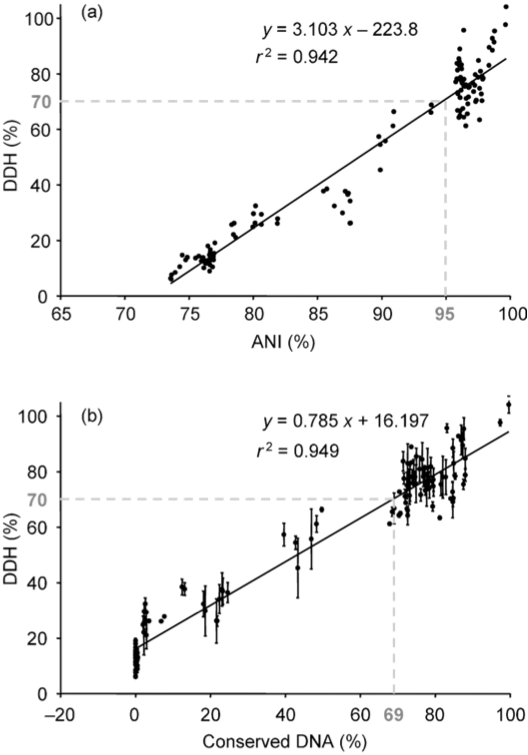
\includegraphics[width=\textwidth]{images/ani_ddh_equiv}
  \end{columns}    
\end{frame}

%
\begin{frame}
  \frametitle{Average Nucleotide Identity (ANI)
  \footnote{\tiny{\href{http://dx.doi.org/10.1073/pnas.0906412106
}{Richter \& Rossell\'{o}-M\'{o}ra \textit{et al.} (2009) \textit{Proc. Natl. Acad. Sci. USA} doi:10.1073/pnas.0906412106
}}}
  }
  ANIm and TETRA variants introduced in 2009:
  \begin{columns}[T] 
    \column{.5\textwidth} 
      \textcolor{RawSienna}{ANIm}
      \begin{enumerate}
        \item \textcolor{hutton_green}{Align sequences with NUCmer (no fragmentation)}
        \item \textcolor{hutton_purple}{ANI = mean identity of matches}
      \end{enumerate}
    \column{.5\textwidth}
      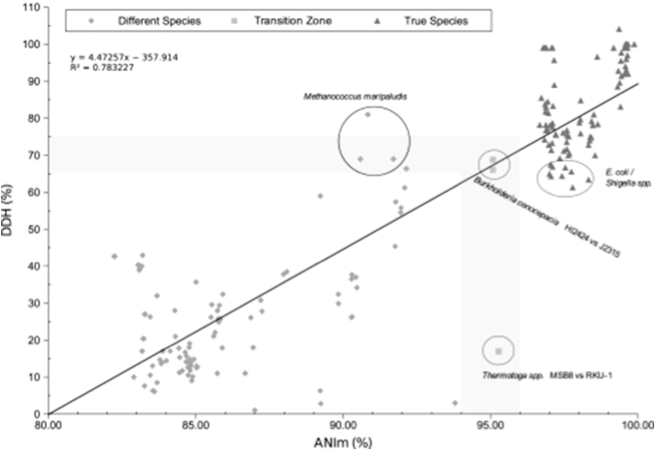
\includegraphics[width=\textwidth]{images/anim_ddh_equiv}
  \end{columns}    
  \textcolor{RawSienna}{TETRA} (a bulk measure!)
  \begin{enumerate}
    \item \textcolor{hutton_green}{Calculate 4-mer frequencies}
    \item \textcolor{hutton_blue}{Determine Z-score for 4-mer deviation from expected value, given \%GC content}
    \item \textcolor{hutton_purple}{TETRA = Pearson correlation coefficient of Z-scores}
  \end{enumerate}
\end{frame}

%
\begin{frame}
  \frametitle{Bulk genome comparisons}
  \Large{
    \textcolor{hutton_blue}{
      \textbf{
      EXERCISE 3: \\
      \url{ex03_ani.ipynb}
      }
    }
  }
\end{frame}

%
\begin{frame}
  \frametitle{Bulk genome comparisons}
  \textit{Anaplasma} spp. comparisons \\~\\
  \begin{columns}
    \column{.33\textwidth} 
      ANIb \\
      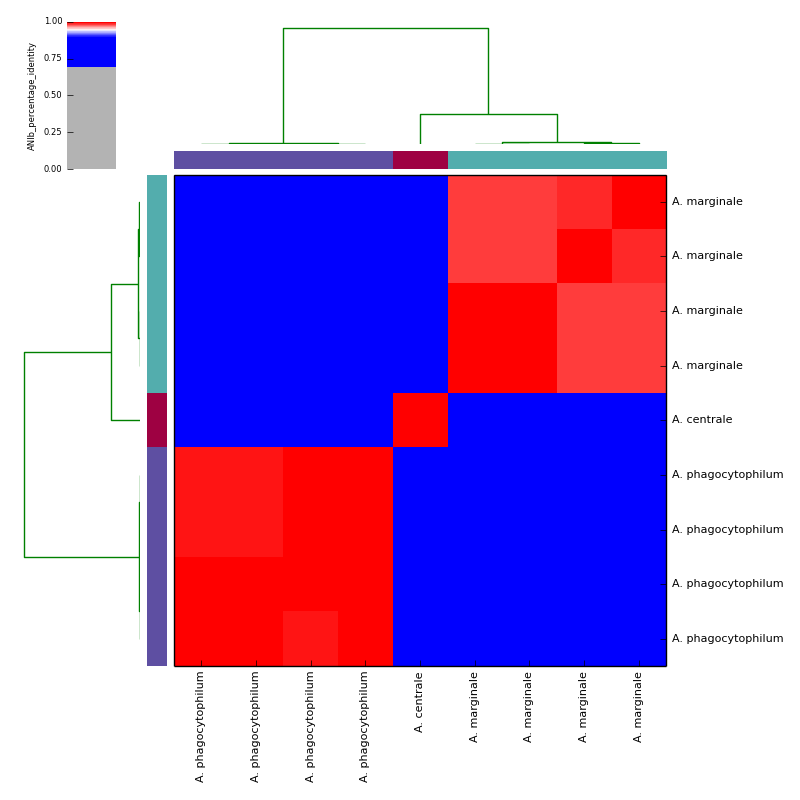
\includegraphics[width=\textwidth]{images/ANIb_percentage_identity}
    \column{.33\textwidth}
      ANIm \\
      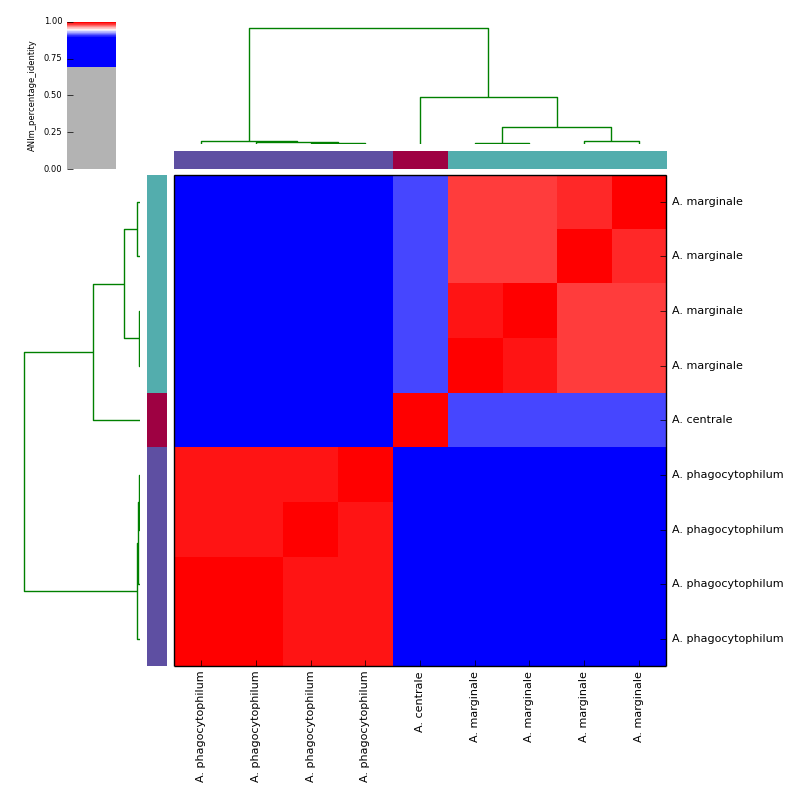
\includegraphics[width=\textwidth]{images/ANIm_percentage_identity}    
    \column{.33\textwidth}    
      TETRA \\
      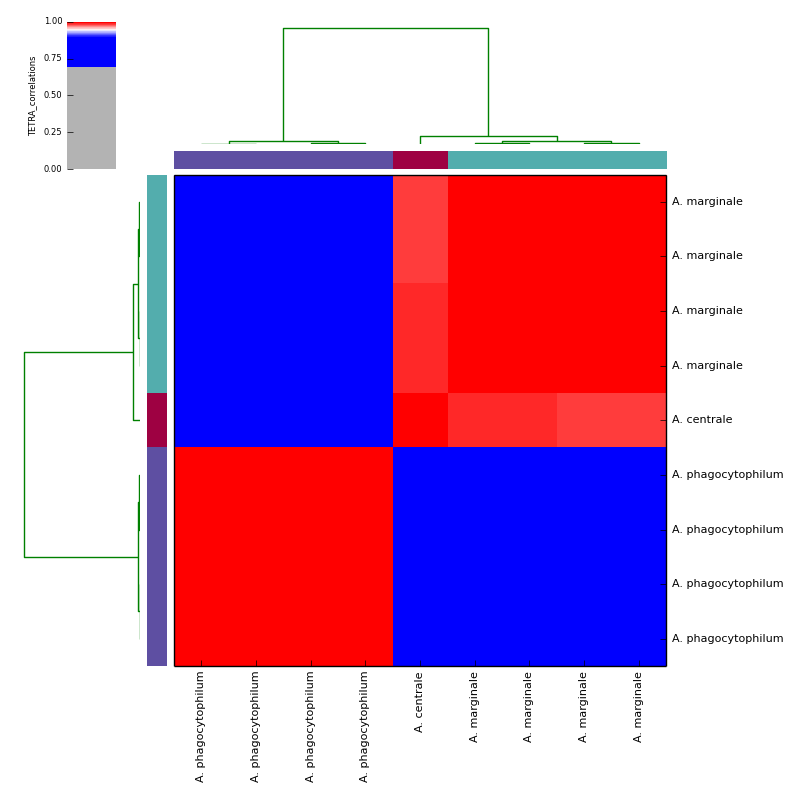
\includegraphics[width=\textwidth]{images/TETRA_correlations}    
  \end{columns} 
\end{frame}

% ANIm in practice
\begin{frame}
  \frametitle{ANI in practice
    \footnote{\tiny{\href{http://dx.doi.org/10.1099/ijs.0.052944-0}{van der Wolf \textit{et al}. (2014) \textit{Int. J. Syst. Evol. Micr.} \textbf{64}:768-774 doi:10.1099/ijs.0.052944-0
    }}}
    }
  \begin{columns}[T]
    \begin{column}{5cm}
    29 \textit{Dickeya} isolates:\\
    species structure\\
      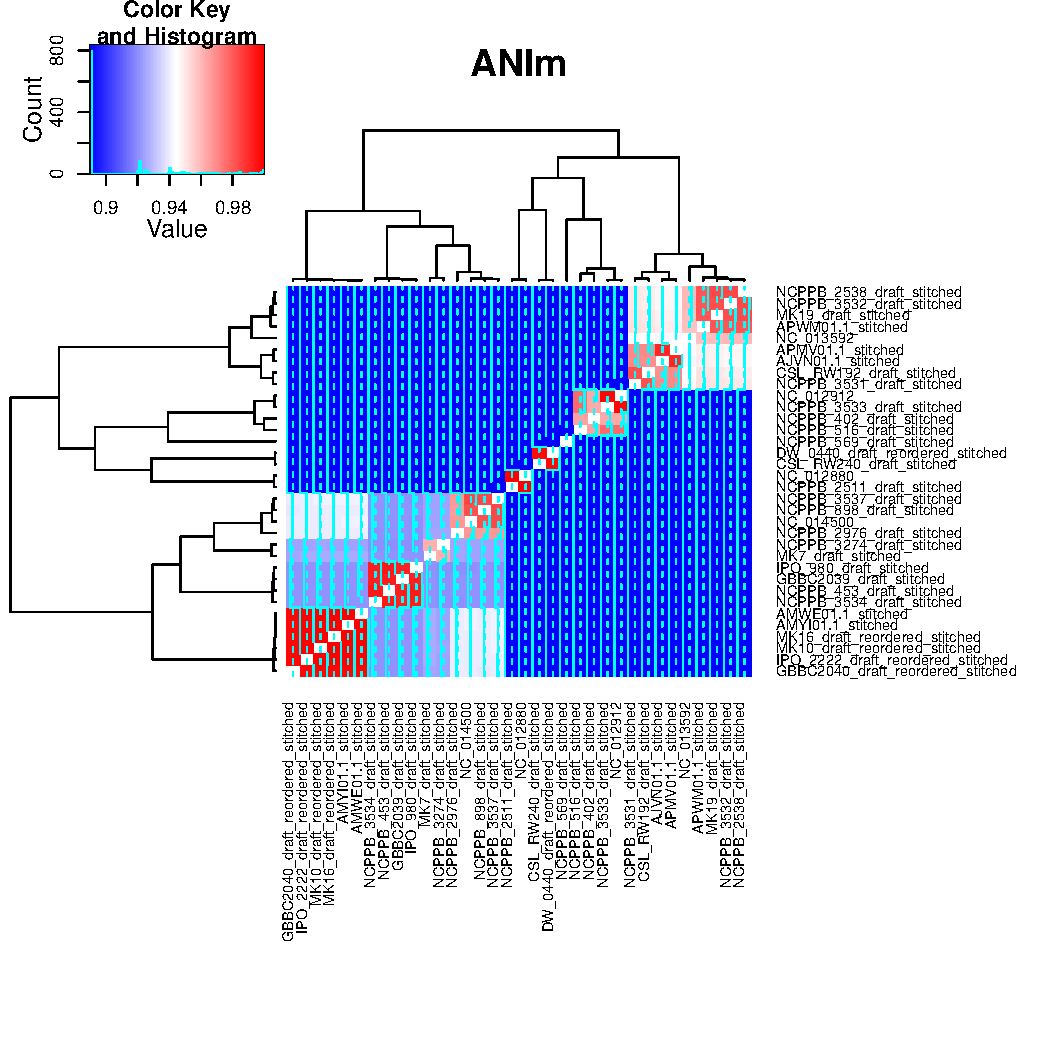
\includegraphics[width=\textwidth]{images/ANIm_Dickeya}
    \end{column}
    \begin{column}{5cm}
    180 \textit{E.coli} isolates:\\
    subtyping
      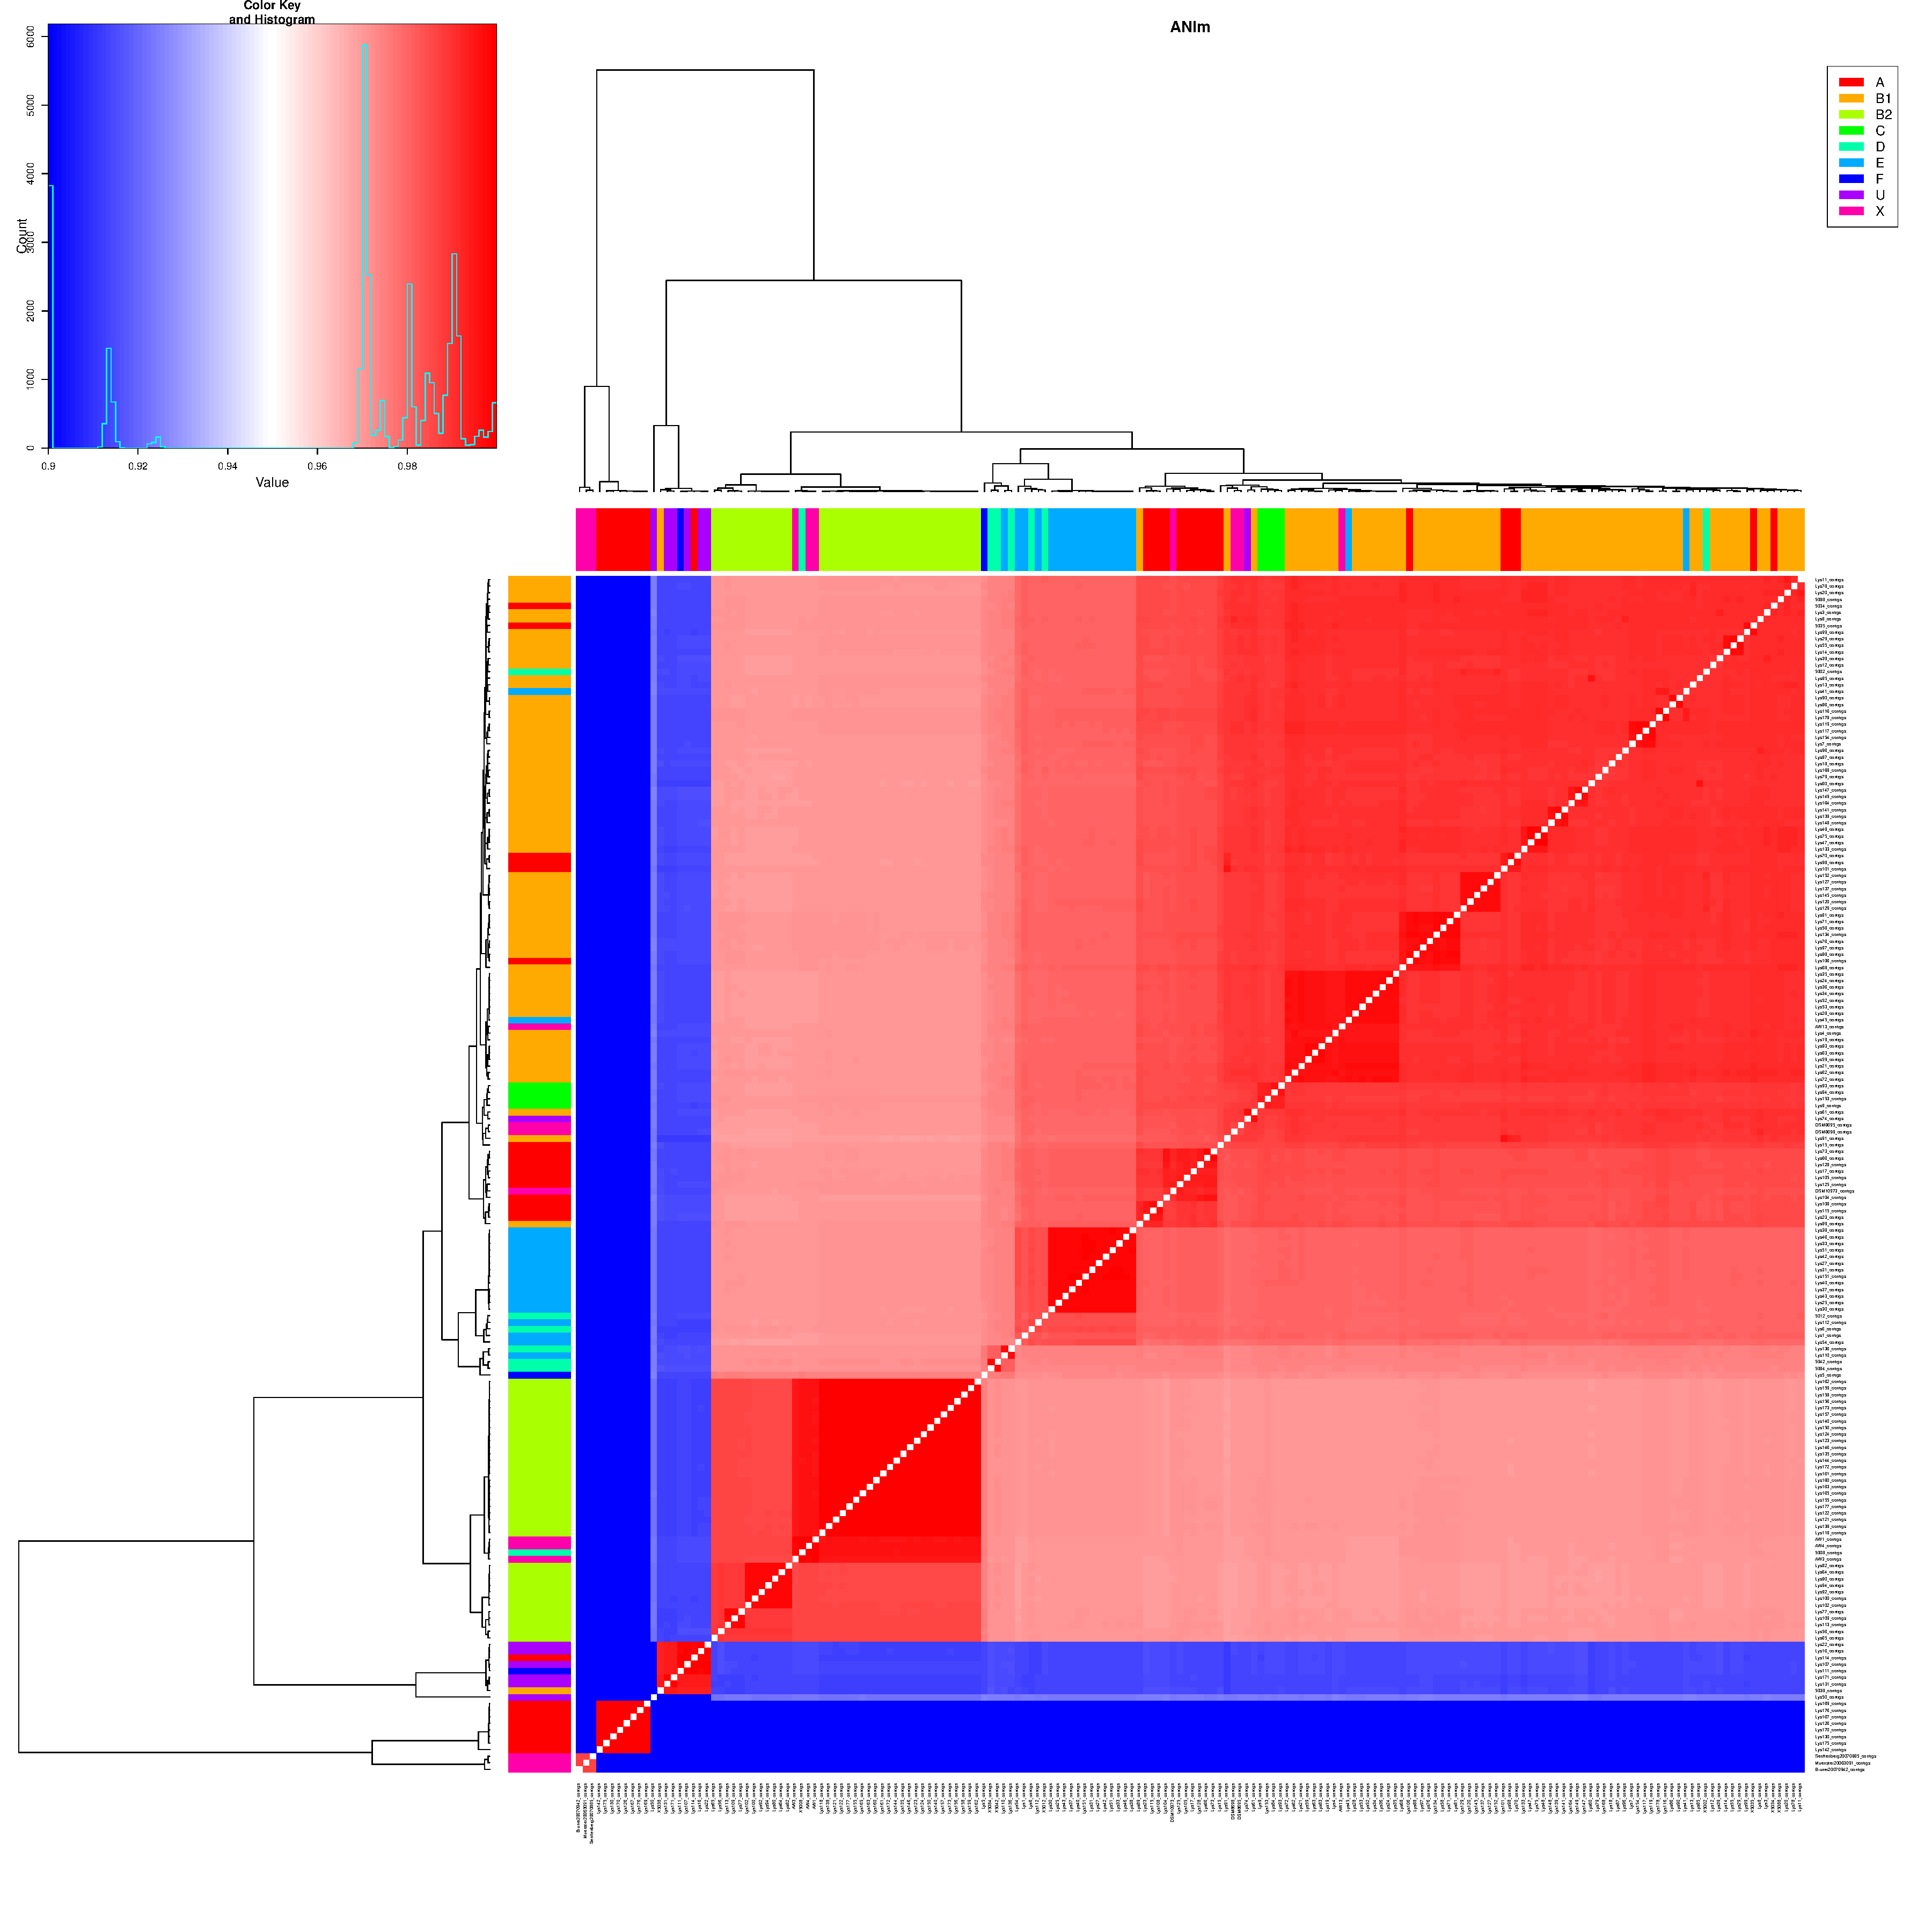
\includegraphics[width=\textwidth]{images/ANIm_Ecoli}
    \end{column}
  \end{columns}       
\end{frame}

%
\begin{frame}
  \frametitle{Average Nucleotide Identity (ANI)}
  \textcolor{hutton_green}{ANIb vs ANIm}
  \begin{itemize}
    \item ANIb can split a single matching region into two fragments that do not match criteria
    \item $\implies$ ANIb may discard useful information that ANIm retains
  \end{itemize}
  \textcolor{hutton_blue}{ANIb/ANIm vs TETRA}
  \begin{itemize}
    \item ANIb/ANIm reflect sequence matching (analogous to hybridisation)
    \item TETRA reflects statistical deviation of a bulk genome measure (4-mer frequency)
    \item TETRA may be prone to false positives (saying two sequences are the same species when they are not)
  \end{itemize}  
\end{frame}
